\documentclass{article}
\usepackage[utf8]{inputenc}
\usepackage{graphicx}
\usepackage{cleveref}
\usepackage{enumitem}

\usepackage{titlesec}

\setcounter{secnumdepth}{4}

\titleformat{\paragraph}
{\normalfont\normalsize\bfseries}{\theparagraph}{1em}{}
\titlespacing*{\paragraph}
{0pt}{3.25ex plus 1ex minus .2ex}{1.5ex plus .2ex}

\title{Final IDP Report}
\author{Group M213 ; Team Name: Roomba PLC ;Robot Name: Roomba}
\date{3rd December 2022}

% To be confirmed that it requires the setspace package, try with and without.
\usepackage{setspace}

% Let top 85% of a page contain a figure
\renewcommand{\topfraction}{0.85}

% Default amount of minimum text on page (Set to 10%)
\renewcommand{\textfraction}{0.1}

% Only place figures by themselves if they take up more than 75% of the page
\renewcommand{\floatpagefraction}{0.75}

%zet de bladspiegel :
\setlength\paperwidth{20.999cm}\setlength\paperheight{29.699cm}\setlength\voffset{-1in}\setlength\hoffset{-1in}\setlength\topmargin{1.499cm}\setlength\headheight{12pt}\setlength\headsep{0cm}\setlength\footskip{1.131cm}\setlength\textheight{25cm}\setlength\oddsidemargin{2.499cm}\setlength\textwidth{16.5cm}

\begin{document}

\maketitle

% TODO: Please fill in your details in the table below

\begin{table}[]
    \centering
    \begin{tabular}{|c|c|c|c|}
        \hline
        Name &  CRsid & College & Lab Group \\
        \hline
        Matthew Hendricks & mah237 & Pembroke & 35 \\
        Louis Pender & lwp256 & Lucy Cavendish & 17 \\
        Hor Ye Heng & yhh35 & Peterhouse & 30 \\
        Wen Yian & yw543 & Pembroke & 39 \\
        Yiheng Liu & yl827 & Lucy Cavendish & 13 \\
        Zhang Yuge & yz754 & Peterhouse & 30 \\
        \hline
    \end{tabular}
    \caption{Coversheet information}
    \label{tab:Coversheet}
\end{table}


\newpage

\section{Introduction}
\quad The aim of this project is to design and build a robot that can navigate along a line track and collect and classify blocks of different densities. The competitions are marked using the following criteria:

\begin{itemize}
    \item Robot first traverses to other side of table (no part of robot on ramp or in tunnel) +10
    \item Robot traverses both ramp and tunnel +10
    \item Block delivered to correct area (entirely within lines) +10
    \item Block transported to delivery side of table +10
    \item Correct LED displayed to identify block +10
    \item Robot finally returns to a start/end box and stops such that the robot is entirely within the lines of the box. The robot must have made a sporting attempt to identify and collect blocks +20 
    \item 1st Competition only manual demonstration of block identification (block may be brought up to stationary robot by hand to demonstrate correct detection reliably) +10
\end{itemize}

\quad The robot must be able to traverse the ramp and tunnel, detect and deliver the blocks to the correct area. By traversing the ramp first before picking up the block, the robot can just push the block on the floor without lifting it which is far easier.

\quad To meet these criteria in the small timeline given our group was organised into mechanical, electrical and software teams. We also used a variety of tools to help us with our project management, design and collaberation.

\quad We made an overall system level diagram as can be seen in \Cref{fig:overall_sys}

\begin{figure}[!h]
    \centering
    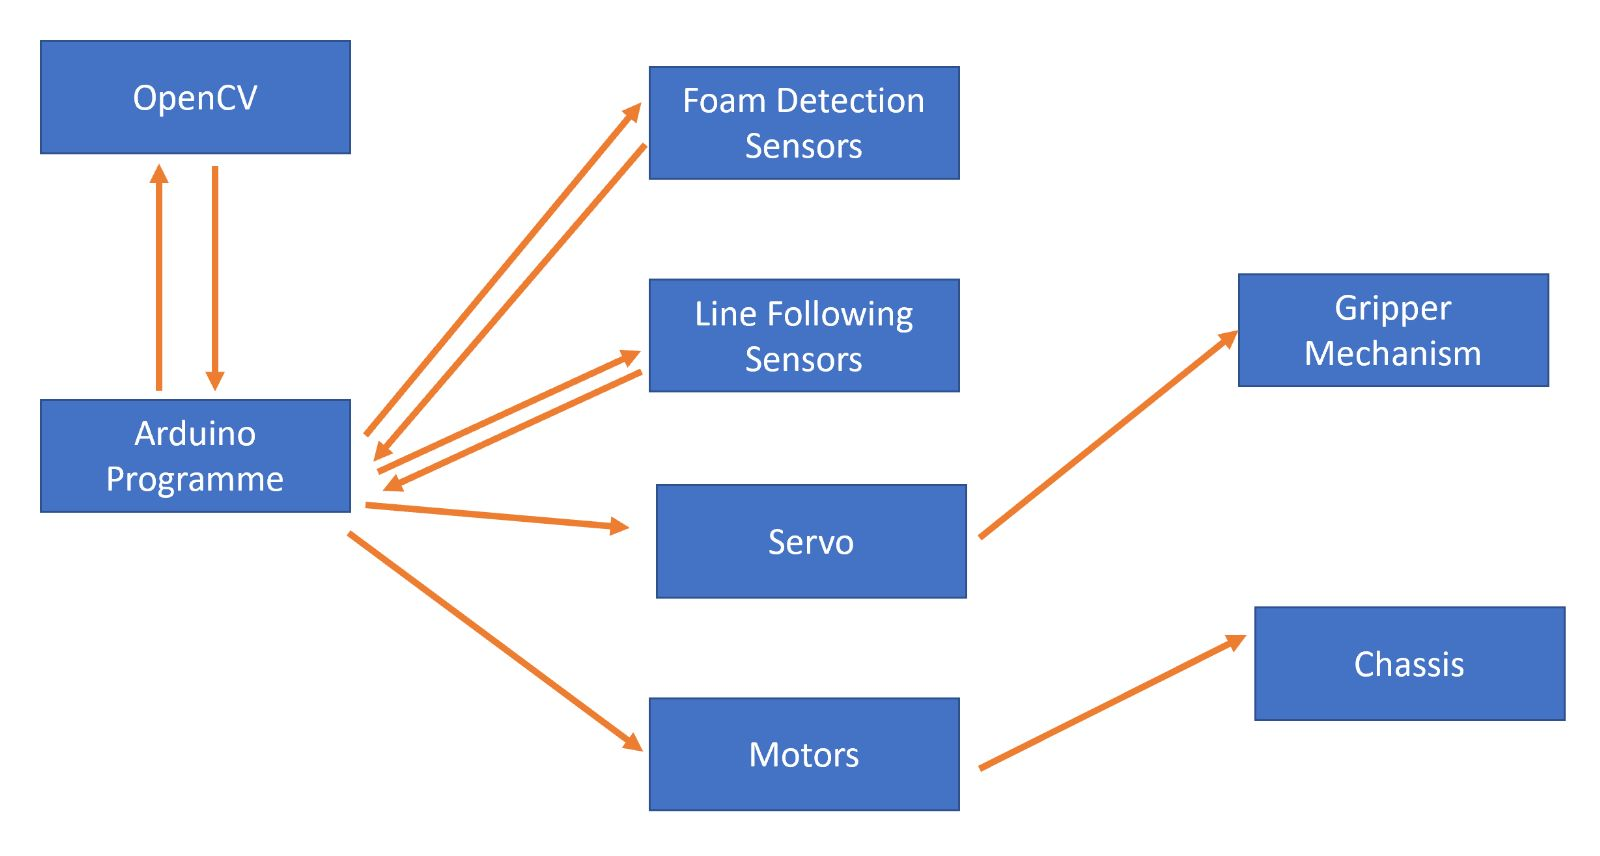
\includegraphics[width=0.8\textwidth]{assets/Overall_sys.jpg}
    \caption{Overall System Level Diagram}
    \label{fig:overall_sys}
\end{figure}

\section{Project Management}
\quad L.W. Pender was selected as the leader of the group. We created a Trello project which has functionalities like a Gantt chart and Kanban boards as our project management systems. We made a rough timeline of the large milestones of the project such as having a fully assembled robot, having the sensors all attached onto the robot and funcitoning, having a working robot and testing, and placed these onto the Trello project. We then made smaller short-term goals for each team to achieve. A Gantt chart for the project can be seen in \Cref{fig:gantt}.

\begin{figure}[!h]
    \centering
    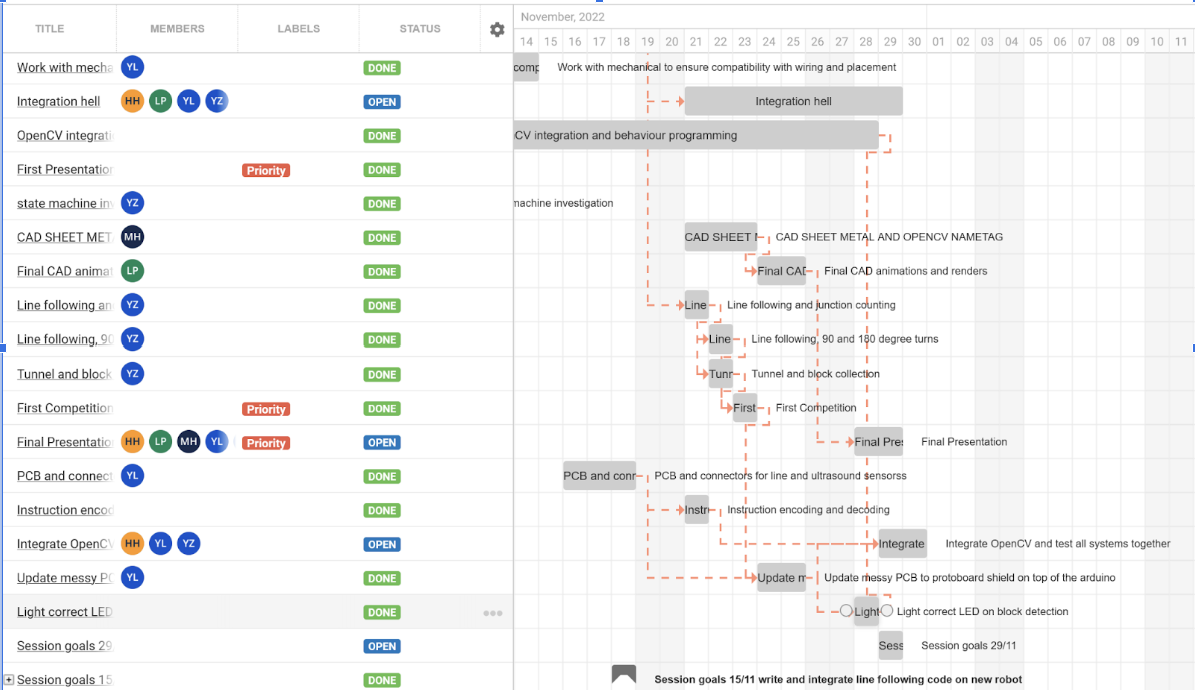
\includegraphics[width=0.8\textwidth]{assets/Gantt.png}
    \caption{Screenshot of Gantt Chart}
    \label{fig:gantt}
\end{figure}
    
\hspace{10em}

\section{Mechanical}
\quad The mechanical team consists of Pender, L.W. (lwp26) and Hendricks, M.A. (mah237). 

\subsection{Drive System}
\quad \quad We initially considered a few drive systems for the robot, namely a 3-wheeled differential drive system, a 4-wheeled tank drive system, making our own Mecanum wheels and a simple 2-wheeled system. 

\quad We ruled out the Mecanum wheels idea due to the sheer difficulty of manufacturing such a wheel without much added benefit to the project since the main priority for our team would be rapid production so that testing can begin sooner rather than later. The 3-wheeled differential drive was also ruled out due to not having 3 same-sized wheels. This is because we don't want the base of the chassis to be inclined in case we would have markers (such as QR codes) used by the software team for navigation and other purposes. The inclination would probably lead to larger errors in navigation. We ruled out the 4-wheeled tank drive system, as we were worried about slipping occuring in one of the sets of wheels if the ratios of the speeds were not accurate. This is especially important to us since we're thinking about using a light sensor as a rotary encoder to have an accurate measure of the distance travelled by the robot. A table summarising our comparisons can be seen in \Cref{tab:drive_comp}.

\quad Therefore, the best option we settled on was the simple 2-wheeled system, since it would be the simplest to manufacture. We plan to use the larger wheels so that our rotary encoder would be more accurate. The wheels will be connected to the higher torque lower RPM motor via the given motor adaptors. The higher torque will help in the robot going up the ramp. The motors will be attached to the robot by a metal bracket and bolting it onto the threads on the aluminium plate on the motor. We also will place a ball castor at the other end of the chassis to ensure the robot remains stable as it ascends the ramp. However due to the line sensors in our final robot being placed too low and too far away from the castor ball, the line sensors end up catching the ramp. There was a tradeoff decision here as fixing this problem would leave less time for the software team to test the robot and might require recalibration. After some discussion with the team, we decided to focus on other aspects of the robot and only use the tunnel so we could get more points more reliably.

\begin{table}[!h]
    \centering
    \begin{tabular}{|c|p{5cm}|p{5cm}|}
        \hline
        Idea & Advantages & Disadvantages \\
        \hline
        2-wheeled + Castor wheel & Fast to manufacture quickly& Might be harder to turn \\
        3-wheeled differential-drive & Easy to manufacture quickly & Might slip since wheels are not of same size \\
        4-wheeled tank drive system & Very reliable & More motors required and hard to sync the motor's rpm ratio due to different sized wheels \\
        \hline
    \end{tabular}
    \caption{Drive System Comparison}
    \label{tab:drive_comp}
\end{table}

\subsection{Chassis}
\quad After looking at the sizes of the various components (such as the Arduino and the battery pack) that we needed to fit onto the chassis we make a rough guess of a dimension of the base of the chassis to be $250mm \times 140mm$ with a top and bottom plate. The bottom plate would hold the battery and the motors (for a lower center of gravity). and the top plate would hold the rest of the electronics. The bottom plate was made out of 6mm plywood and the top plate out of 3mm plywood to further lower the center of mass.

The chassis design for the robot was designed to be very modular, we had multiple holes for the components fitting locations so that we can swap the positions of the sensors and other components easily to redistribute the mass in the robot. The parts were laser cut instead of handsawed because it is faster and it gives more precise cuts.

\subsection{Sensor and Peripherals Mounting}
\quad Our group wanted the flexibility to test up to 4 different ways of block detection and differentiation and we built the robot to accomodate all the sensors and peripheral devices required for those detection methods. The 4 methods and their mounting methods are listed in \Cref{tab:mount_sens}. Many of these sensors and mounts were removed in the end as we settled with OpenCV for our navigation method and the LDR method for our detection method, however the flexibility our design provided to the testing process of our team was very valuable.

\begin{table}[]
    \centering
    \begin{tabular}{|c|p{5cm}|p{5cm}|}
        \hline
        Detection Method & Sensors Required & Mounting Method \\
        \hline
        Ultrasound sensing & Ultrasound sensor and IR Sensor & 3D Printing Brackets and bolting \\
        \hline
        Testing Motor Current & Grabbing Mechanism & Bolted with washers and spaced with nuts.\\
        \hline
        LDR reading & LEDs and LDRs on grabbers & fit LEDs into precise holes and bolted heat shrinked regions of the LDR wire \\
        \hline
        OpenCV sensing & LEDs shining light on the cube & Made metal bracket at the top of the chassis.\\
        \hline
    \end{tabular}
    \caption{Sensor and Peripheral Mounting}
    \label{tab:mount_sens}
\end{table}

\subsection{Gripping Mechanism}
\quad We had 3 main ideas on how to capture the block. 

\quad The first was a simple pushing idea where we had a slight protrusion at the edges of the robot to ensure it doesn't get pushed off the robot. However this not only limits our route to be leaving the collection arena from the tunnel, it also is not reliable during turning.

\quad The second idea was to have a rack and pinion powering a moving stick to move closer to another stationary stick to grab the block. The problem with this was that the rack and pinion mechanism is less reliable and the block will be gripped to one side of the mechanism and the mass distribution will be shifted.

\quad The idea we settled on was to use a scissor like gripping mechanism. This might have slightly more parts but it is more reliable than the rack and pinion and the center of mass is not affected. This also had the great benefit of only using one servo.

\subsubsection{Assembly}

\quad The assembly of the grabber mechanism required the use of pin joints to allow the parts of the mechanism to rotate and grab the block. We made the pin joints by having bolts separate the pieces with nuts and washers so that the joints will have less friction and will act like a pin joint. Another problem we faced during assembly was that the parts did not mesh together really well because of the difference in heights of the parts and the robot chassis being slightly warped due to some bolts joining the top and bottom plate together. We resolved this by having a long bolt through the top and bottom plate and used nuts fix the distance from the top to the bottom plate near the grabber. This ensured that the grabber gears meshed well together.

\subsection{Cardboard Model and CAD}
\quad We have made a cardboard model prototype for testing purposes. This was laser cut out of cardboard and assembled using hot glue. Our first wooden robot was produced fairly quickly but was determined to be the final robot instead of reproducing another one to allow the other teams to continue testing the robot which was more critical to the project at the time.

The CAD model of the final robot and some drawings can be seen in \Cref{fig:cadndraw}.

\begin{figure}[!h]
    \centering
    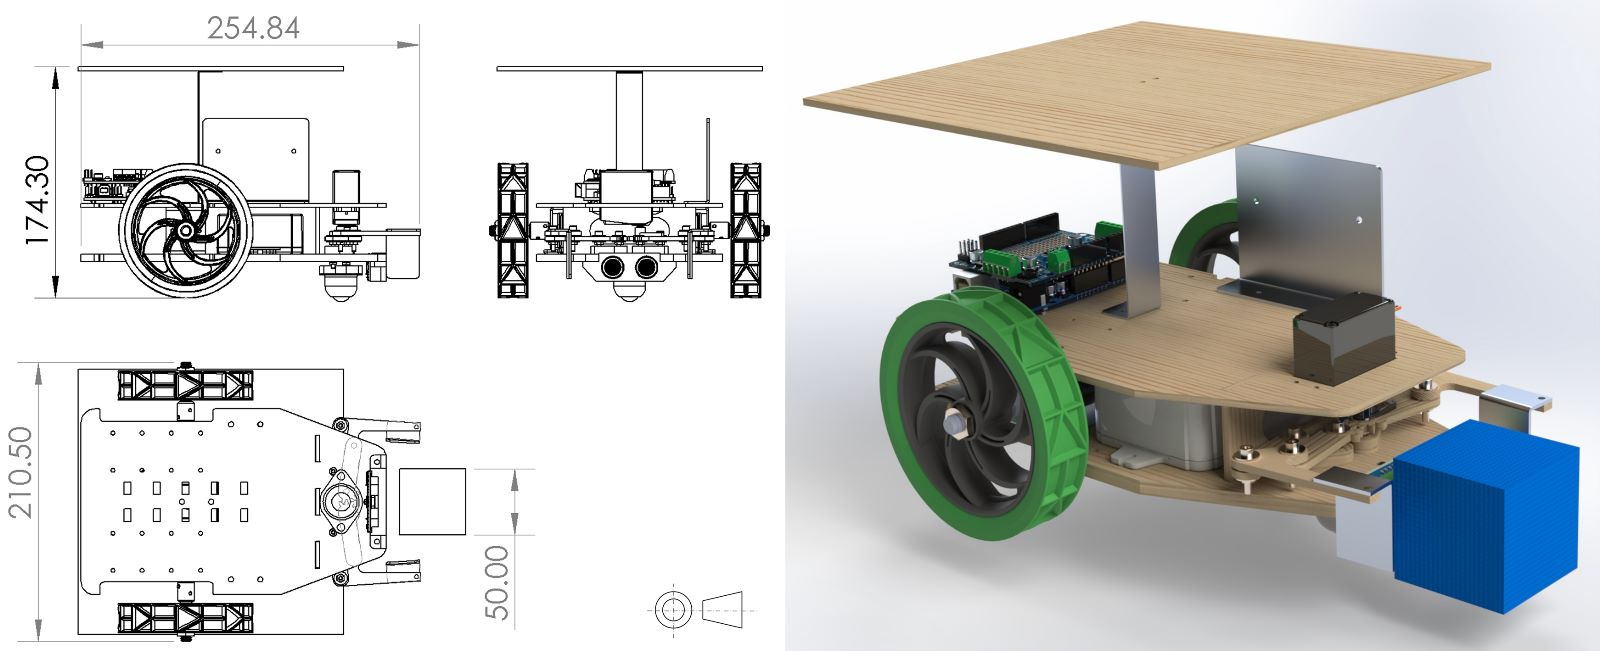
\includegraphics[width=0.8\textwidth]{assets/CAD_ndrawing.jpg}
    \caption{CAD and Drawings}
    \label{fig:cadndraw}
\end{figure}

\section{Electrical}
\quad The electrical teams consists Ye Heng Hor (yhh35) and Yiheng Liu (yl827)

The electrical design went through significant changes throughout the development lifecycle of the project, because we decided to transition to computer vision for navigation after the first competition, which greatly simplified the electronics.

For completeness, a brief overview of everything implemented, regardless of whether or not they were used in the final implementation, is included below.

\subsection{Line Following}
\subsubsection{Component List}
The line following robot contains the following components, and their functions are shown in \Cref{tab:elec_comp}

\begin{table}[!h]
    \centering
    \begin{tabular}{|c|p{5cm}|p{5cm}|}
\hline
Component &
  Function &
  Implementation
   \\
   \hline
Line Sensor (OPB704) &
  Provides a voltage readback representing the infrared reflectance of the surface below. &
  Connect in series with resistors to give a feedback voltage to the Arduino according to surface detected
   \\
   \hline
Ultrasonic Sensor &
  Send pulses and receive echo of the pulse to determine distance from obstacle &
Connected to PWM port of Arduino to send pulses  Time the difference between pulse and echo by Arduino to determine the distance from wall and obstacle (block)
   \\
   \hline
Light Dependent Resistor &
  Changes resistance according to amount of incident light, which changes with block density &
  Connect in series with resistors   to give a voltage to Arduino according to light shine (reflection from block) 
   \\
   \hline
LED &
  Indicates robot state &
4 white LEDs connected in series with 100ohm resistor to shine up block Amber/Green/Red used to indicate   working state\\
  \hline
    \end{tabular}
    \caption{Component List}
    \label{tab:elec_comp}
\end{table}

\subsubsection{Schematic and PCB layout}
\quad The schematic is shown in \Cref{fig:sche}.

\begin{figure}[!h]
    \centering
    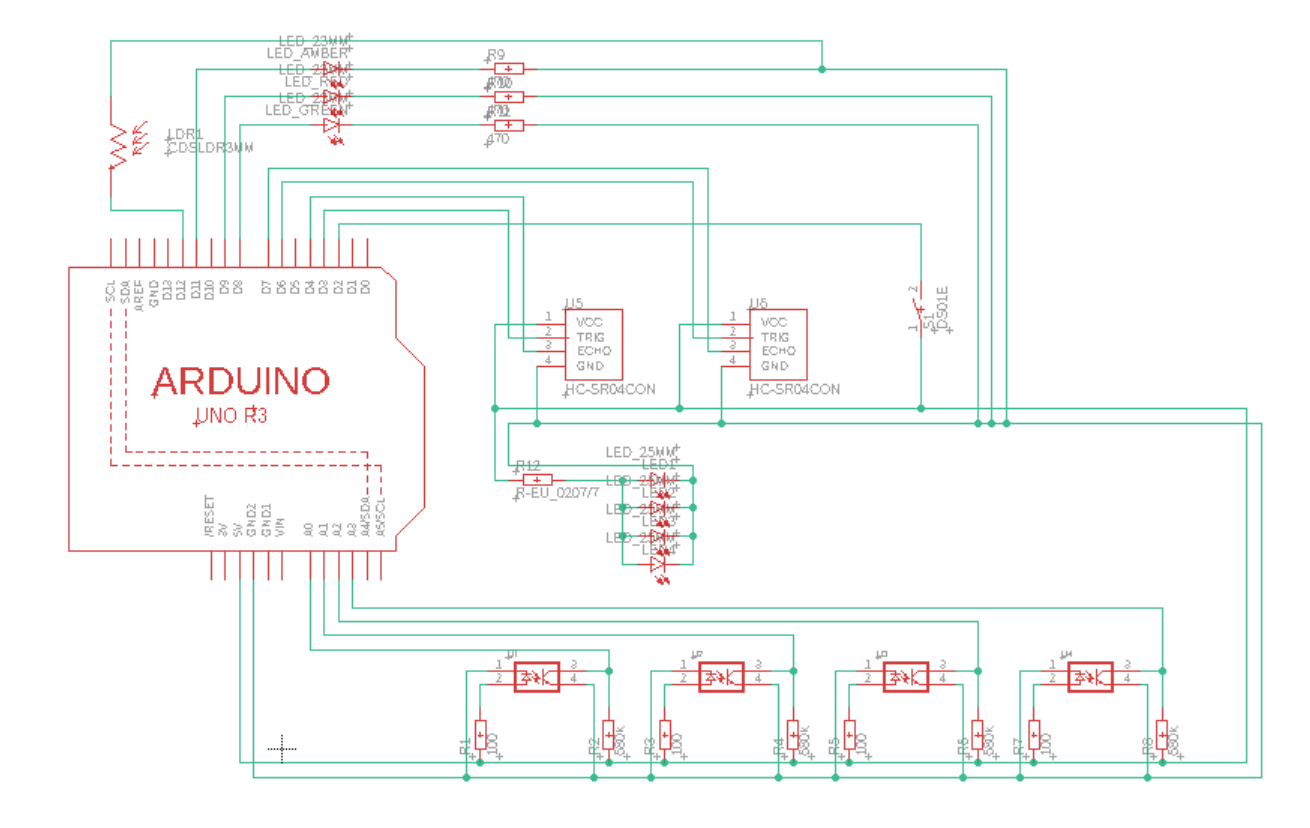
\includegraphics[width=0.8\textwidth]{assets/Schematic.png}
    \caption{Schematic Diagram}
    \label{fig:sche}
\end{figure}
These were all done soldering in week 3 and ready for test on stripboard. We originally used stripboard to build our circuit as it is faster to prototype and change any designs according to tested results. Functions are all tested fine before installed to the robot.
As the four line sensors occupied all analog inputs on the arduino, we implemented code in software to make pin 12 capable of reading analog inputs and have the LDR connected to it.

However, it became apparent on the morning of the first competition that the exposed pads on the board were shorted by exposed nuts on the robot frame, causing one of the line sensors to completely malfunction, which caused the robot to only be able to score 20 points, since we could not navigate back to the starting half of the arena.

We made the decision to use the Arduino shield boards, as they would completely eliminate shorting of component pads by coming into contact with random metal surfaces on the robot. This really helped to ensure that the robot's performance was robust and reliable.
\begin{figure}[!h]
    \centering
    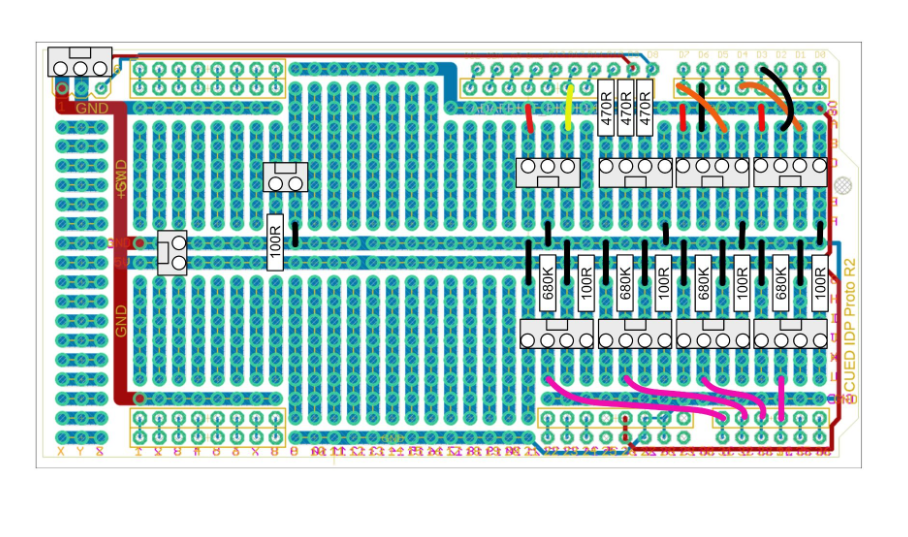
\includegraphics[width=0.8\textwidth]{assets/Proto.png}
    \caption{Board Layout Diagram}
    \label{fig:bldiag}
\end{figure}
\begin{figure}[!h]
    \centering
    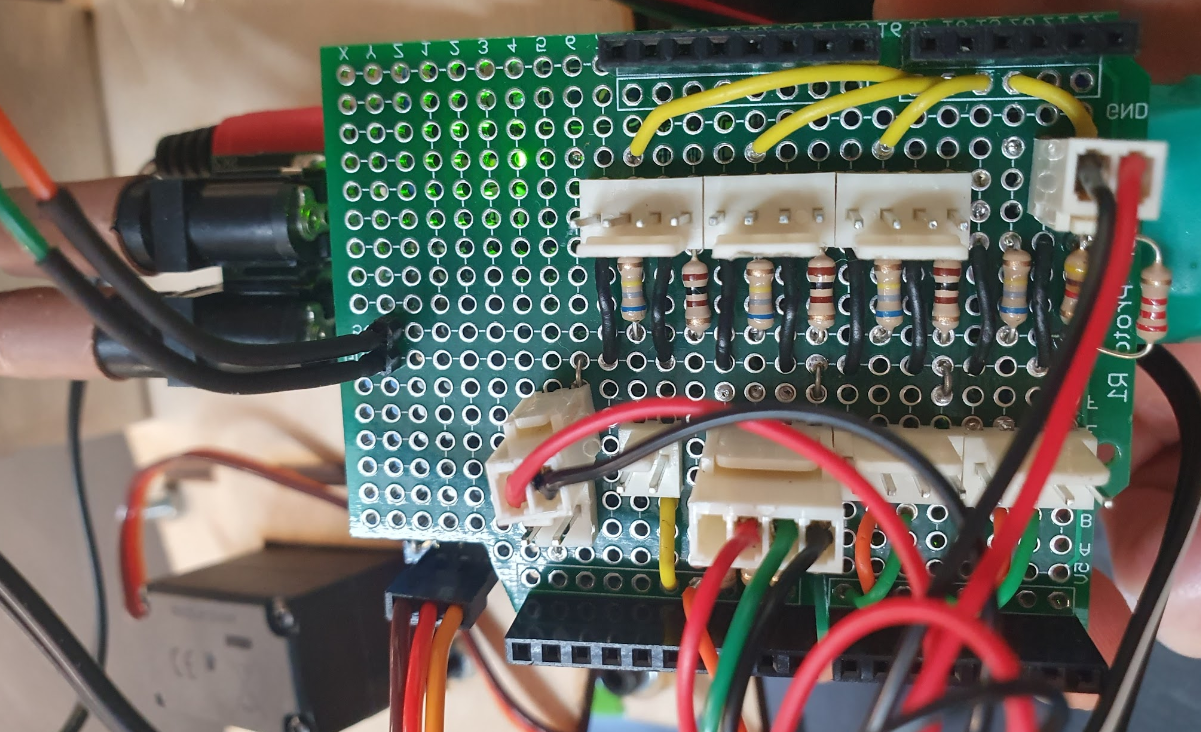
\includegraphics[width=0.8\textwidth]{assets/Board.png}
    \caption{Completed Board}
    \label{fig:cbldiag}
\end{figure}

\quad As we made the decision to make the change to OpenCV, most of the sensors were no longer needed. Only the LDR, which is used for detecting block density, remained.

Thus, the only change to the PCB is LDR now connected to A3 to ensure stable performance, as line sensors are no longer required. The rest of the connectors are left unpopulated.

\section{Software}

\quad The software team consists of Yian.W (yw543) and Yuge.Z (yz754). For software, there are two separate systems proceeding at the same time: Line-following and OpenCV (explored by Ye Heng Hor (yhh35)). Th initial intention was to have separate systems that could either work in conjunction with each other for redundancy, or to pick whichever produces the more complete/stable end result.
\subsection{Line Following design}
The line following design includes the following:
\begin{itemize}
    \item 4 line sensor at the bottom of robot would give voltage values for black and white floor. We set up threshould values for low/high states, and then design the basic line-following logic.
    \item 2 distance sensors are installed in front and right hand side of the robot separately. The front one detects the block, and the side one detects the wall in tunnel.
    \item The ultrasonic sensor in front of the robot detects the density of the block.
\end{itemize}

The main logic (which involves the detection from sensors) for the system is: Follow the white line with correction. If inside tunnel (when all line sensors give low reading), correct the movement with side distance sensor's reading.
If the front distance sensor detects the block, stop the robot, detect the density and return to corresponding square. Then go home. We plan not to go over the ramp due to some mechanic issue, and all of these if conditions are ensured to be triggered correctly with time counted.

\subsubsection{Test and trade-off in design}
The tests show that the line-following function works perfectly. However, the front ultrasonic and distance sensors do not work ideally. For ultrasonic sensor, it does not give reliable reading for block density. While for distance sensor, it is the problem of position it is installed.
The distance sensor is installed towards the floor rather than towards the front, which sometimes accidentally trigger the "block detected" function.

The problems of sensors cannot be solved effectively and as a result, we can only count the time to stop the robot, trigger "pick up" function and then return, sacrificing the maximum number of blocks got and aim for only one block.

\subsection{OpenCV}
\subsubsection{Decision to abondon line following}
We made the decision to attempt to use OpenCV for the following reasons:

\begin{itemize}
    \item To allow the robot to traverse the ramp, significant, potentially breaking changes would need to be made to the location of the line sensors
    \item The electrical connection to the line sensors have been rather unreliable.
\end{itemize}

\subsubsection{OpenCV Control Architechture}
The main control loop brings together the following 2 modules to complete the tasks set by CUED:

\paragraph{Remote Control over Wifi}

A http request parser was implemented on the Arduino onboard the robot, which allows for a master-slave style communication protocol. 

The Arduino is connected to the main control PC via the PC's mobile hotspot. The PC can then send commands over to the Arduino, each consisting of an instruction string and an optional parameter string. For example, the robot can be commanded to \textbf{move forward} for \textit{1000ms}. After each command, the Arduino sends back a HTTP 200 OK response, with a reading of the LDR value, which enables the detection of the block type.

\paragraph{Video Acquisition and Processing}
The video acquisition module takes care of tasks like acquiring real time video from the overhead camera, correcting for distortion and locating the robot.

The `arena` class located within this module also contains calibrated waypoints for navigation across the arena, which include all the positions where blocks are to be collected or dropped, as well as tunnel and ramp endpoints.

\paragraph{Control Loop Behavior}
At the beginning of the routine, a calibration is performed where the distance and anglular displacement per unit time is recorded, and used for all subsequent movement commands.

Then, the robot simply navigates to predetermined waypoints and performs the requisite actions to complete the tasks set for us.

\paragraph{Scheme to Improve Reliability}

Due to the script losing track of the marker intermittently when the robot is at the peripheral areas of the camera, and by extension the very edges of the arena, we devised the following scheme to attempt to regain a lock on the AruCo marker:

When the main control script requests a reading of the current position of the robot, if the target locating script does not manage to find the target in the current frame, it will try again by acquiring a new frame and running all the detection routines on the new frames, for a maximum of `max-retries` times. This helps to solve issues related to missing the marker due to noise.

Should the script still fail to locate the marker, the robot performs a manoevure to attempt to go to an area of the arena where the target has a better chance of being detected. This is achieved in the final script by reversing the robot for 1000 ms and commanding it to go forward for 2000 ms. During our testing, it was found that this reverse before moving forward scheme was particularly effective if the robot gets stuck inside the tunnel.

\subsubsection{Key Decisions in OpenCV Architechture}

\paragraph{Waypoint Based Navigation}

Initially, a complete set of functions to automatically detect features within the arena and intelligently pathfind around was developed. Despite having a working solution, we chose to abandon it in favour of a simpler, pre-recorded waypoint based navigation solution due to difficulties testing the smart feature detection based solution as it requires the arena to be completely clear of unexpected objects, and it was impossible to clear the arena as other teams also had to use it.

\paragraph{Time Based Control}

As the decision to use OpenCV was made rather late, it was not possible to realise the initial idea of having optical encoders on the wheels for absolute position sensing. This made the task of accurately navigating the robot extremely challenging due to the inconsistent performance of the DC brushed motors being controlled by PWM in an open loop manner. However, it was the only option given the time constrains.

\paragraph{Use of AruCo Markers}

Initially, the plan was to use a round target to serve as the main detection target, as a large round object would be very easy to detect since it will be a unique feature within the field of view of the camera. However, upon testing, the size of target needed exceeded our expectations, and 3D printing a target large enough would not have been possible within the time we had. So, the decision was made to use AruCo markers which had the added benefit of also providing information of the heading of the robot.

\paragraph{Only Attempting one lap}
Given the constrains of having to slow down the motors to reduce errors caused by inconsistent motor drive strength, we had to reduce the motor speed to about $80\%$ of maximum, which did not allow us to comfortably navigate around multiple times within 5 mins. Hence, it was decided that we would prioritise getting back to the home point to confidently gain the 20 points associated.

\subsubsection{Failure Analysis}
Unfortunately, despite all the measures described above attempting to increase the reliablilty of the system, it failed to complete a single lap around the arena, which only allowed us to score 10 points out of the (conservatively estimated) 70 points.

The main cause of failure was that the video processing script lost track of the marker, and all of the logic implemented to attempt a recovery failed to do so.

It was particularly perplexing because when the failure occured, the robot was in an area of the arena that had extremely reliable marker detection in all of the prior testing (usually, the marker would be lost near the tunnel edge, but this time the failure occured at the ramp end, which was well within the field of view).

Without extensive testing and validation, it would be hard to conclude what exactly caused this unrecoverable failure. However, by observing the recorded video feed of past successful attempts, and the live video feed as the competition.

\paragraph{Change in Lighting}
We did not expect this to be an issue, as the entire idea of using the monochromatic AruCo marker was that it would be robust against changes in lighting. However, upon scrutiny, the reflections on the tape residue on the arena was different in the recorded and live footage. Considering the marker was printed with a laser jet printer which produces black areas which are glossy, it is possible that somehow light from unexpected sources was reflecting off the marker, causing too much loss of contrast.

The fix for this would be trivial: print the pattern using an inkjet printer, which produces matte prints

\paragraph{Recovery Manoevure was Ineffective}

The recovery manouvre described was great in getting the robot unstuck from under the tunnel, and sometimes effective in enabling the script to regain a lock on the marker. However, in hindsight, the occasions where recovery was achieved when the robot was not stuck were probably flukes, since in the case of the competition, it so happened that the manoeuvre caused the robot to move *away* from the center where detection was most reliable.

A much better way to implement such a recovery measure would be to keep a log of the past commands sent to the robot, particularly those telling it to translate, and send the scaled down reverse of those commands, essentially partially undo-ing the past command that caused the robot to veer out of the zone where detection can be done successfully.

\paragraph{Imbalance in Left and Right Wheels}
This was a known issue since the start of development, and a mitigation was attempted by manually tuning the power sent to each motor, the calibration procedure at the start of the routine, and separating translation and rotation commands (because wheel speed imbalances primarily cause unexpected rotation). However, that still proved to be insufficient.

The best and most straightforward way to solve this problem would be to implement optical encoders on the wheel, as another group did, and as planned for ourselves. This would have the added benefit of increased speed and accuracy, since the movement of the robot would be precisely known, and the slow calibration and on-the-fly heading correction can both be eliminated.

\paragraph{Poor Choice of Pattern}
Looking at another group which managed good results with computer vision, we suspect that the particular pattern index we chose, and thus the generated pattern, was too complex.

Scrutinising the image from the camera revealed that at the periphery of the field-of-view, due to *comatic aberation*, the square cells of the pattern were no longer square, and there was significant spillover of the white areas into the black areas. We suspect that this was the most direct reason the detection was unreliable at the edges of the arena.

This is significant since the marker identification function implemented by the OpenCV library rejects markers that have a certain percentage pixels within cells (squares) which are the wrong colour.

The fix for this would be to choose a marker which is more blob-like, i.e. a marker that contains a large contiguous shape, as the other group had, would probably be more tolerant in terms of this failure mode, than the one we had, which was significantly more checkerboard-like.

Ultimately, these are just educated guesses at why the robot failed the way it did. Despite that, these speculations should serve as excellent jumping off points for any subsequent debugging efforts.

\section{Conclusion}
    \quad We did not manage to achieve our target of 100 points in the competition. The main point of failure was due to the failure of the OpenCV program to detect the robot's position at certain points due to the changed lighting during the competition. Suggested improvements to the development of a robot of this sort would be to make a risk matrix to assess the likely points of failure and perform mitigating actions to prevent them.



\end{document}
